\chapter[Experimental setup]{Experimental setup}

At CERN the high-gradient test are carried on the three X-band test stands (XBOXs), that are setups able to provide the necessary high power RF pulses to the structure under tests. Nevertheless for the tests described in this work the presence of the beam inside the accelerating cavity is necessary, and is provided by the electron linac of the CTF3. 


\section[Linac and dogleg]{Linac and the Dogleg}

\subsection[The test setup]{The test setup}
As mentioned in the first chapter, the main goal of the CTF3 is to demonstrate the feasibility of the CLIC acceleration scheme. For this reason, the linac is used to simulate the Drive Beam to send to the prototypes of Two-beam modules after the recombination process. The linac is realised using the conventional 3 GHz technology, that after the recombination process will lead to the beam frequency of 12 GHz. 

Given that the tests of high-gradient cavities is not the design goal of the facility, in the following sections only the relevant part of the setup for the brakdown experiments will be described. The full description of the CTF3 accelerator complex is widely described elsewhere \cite{CLIC:cdr,CTF:drive_beam,ctf3:dr}.

To realise high-gradient structure tests, a beam line parallel to the linac have been set up. The two beam lines are connected by an oblique segment, giving the characteristic shape that is the origin of the name \textit{Dogleg}.

For the high-gradient testing purpose the accelerator is operated simulating the Main Beam. The parameters of the beam that is possible to produce are reported in the table \ref{beam_par_dogleg}


\begin{table}
  \centering
    \begin{tabular}{ c l }
    \hline
    Current 		&	up to $1.6\,A$\\
    Pulse length		&	up to $250\,ns$\\
    Energy			&	up to $130\, MeV$\\
    Reptition freq.	&	$0.83\,-\,50\, Hz$\\

    \hline
    \end{tabular}
\caption{Beam parameters achievable in the Dogleg \cite{NavarroQuirante:2025954}}
\label{beam_par_dogleg}
\end{table}



\subsubsection{Injector}

The production of the beam is realised by a 140-kV thermoionic gun, designed to deliver up to $5\,A$ of current in nominal operation conditions.
The gun is followed by a S-band prebuncher and a 17 cell travelling-wave buncher. These structures are followed by two 1-m long accelerating structures. The beam dimension in this initial phase is controlled using solenoids, that continue up to the second accelerating structure \cite{ctf:injector}.

Downstream the injector a magnetic chicane with collimators is installed to eliminate off-energy particles and to perform the bunch compression  \cite{Braun:999488}.

The layout of injector and chicane are reported in figure \ref{injlayout}.

\subsubsection{Linac}

In the linac are installed three modules composed of two S-band accelerating structures operating at 3 GHz. The accelerating structures consist of 32 regular cells, operating in the $2\pi/3$ mode. The damping of HOMs is guaranteed by the radial slots in the iris containing SiC loads. The structures are designed for the fully loaded operation with a current of more than 4 A, but when simulating the Main Beam the current is significantly less, implying less loading. In this condition the energy gain is essentially bigger compared to when the Drive Beam is simulated.

The focusing is realised by triplets of quadrupoles, coupled with dipole correctors. The beam energy can be measured in the spectrometers in sector 4 and 10.

The layout of the linac is reported in figure \ref{linaclayout}

\subsubsection{The dogleg}

After sector 7 in the linac, another triplet of quadrupoles is located on the beamline before a bending magnet. When the bending magnet is on, the beam is directed in the dogleg, passing through an oblique section, to end up in a segment of the beamline parallel to the linac. The optics of the dogleg beamline is designed to correct the dispersion provoked by the bending magnets. At the end of the dogleg line the structure under test is placed between two Beam Position Monitors (BPMs). Just before the structure is placed a slit, in order to protect the coupling cell of the structure from being hit by a misaligned beam. The beam is dumped downstream the structure.

In case the first bending magnet is off, the beam proceeds straight in the linac, passing through a triplet of quadrupoles in section 9 and another triplet in sector 10. After that is placed a spectrometer to measure beam energy and momentum. 

The linac proceeds with other accelerating structures, that are not interesting for the development of this work.

The layout of the dogleg and of the linac up to section 10 is reported in figure \ref{dolaut}.


% FIX LAYOUT IN FIGURE 4.3


\begin{landscape}
\begin{center}

\begin{figure}
\centering 
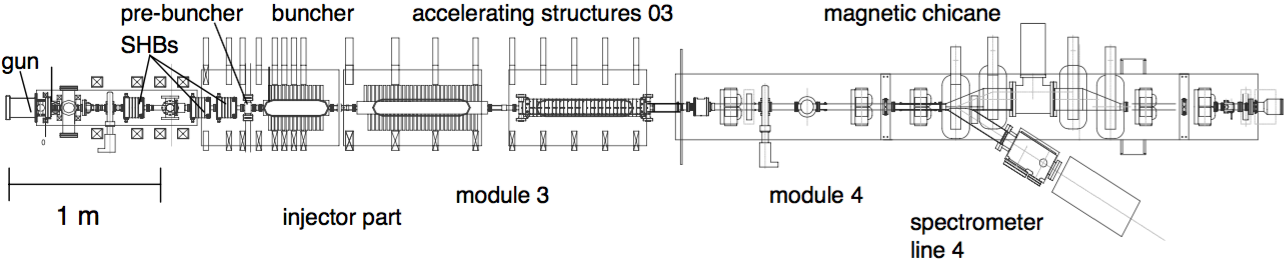
\includegraphics[width=23cm,keepaspectratio]{pictures/Injector}
\caption{Layout of the injector and the magnetic chicane}
\label{injlayout}
\end{figure}

\vspace{20mm}

\begin{figure}
\centering 
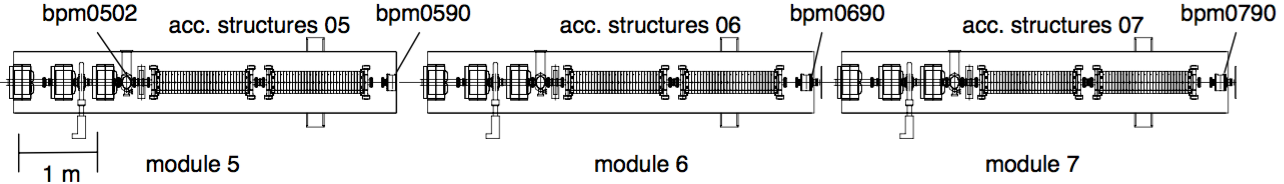
\includegraphics[width=23cm,keepaspectratio]{pictures/girder5-7}
\caption{Layout of the linac up to module 7}
\label{linaclayout}
\end{figure}

\end{center}
\end{landscape}



\begin{landscape}
\begin{figure}
\centering 
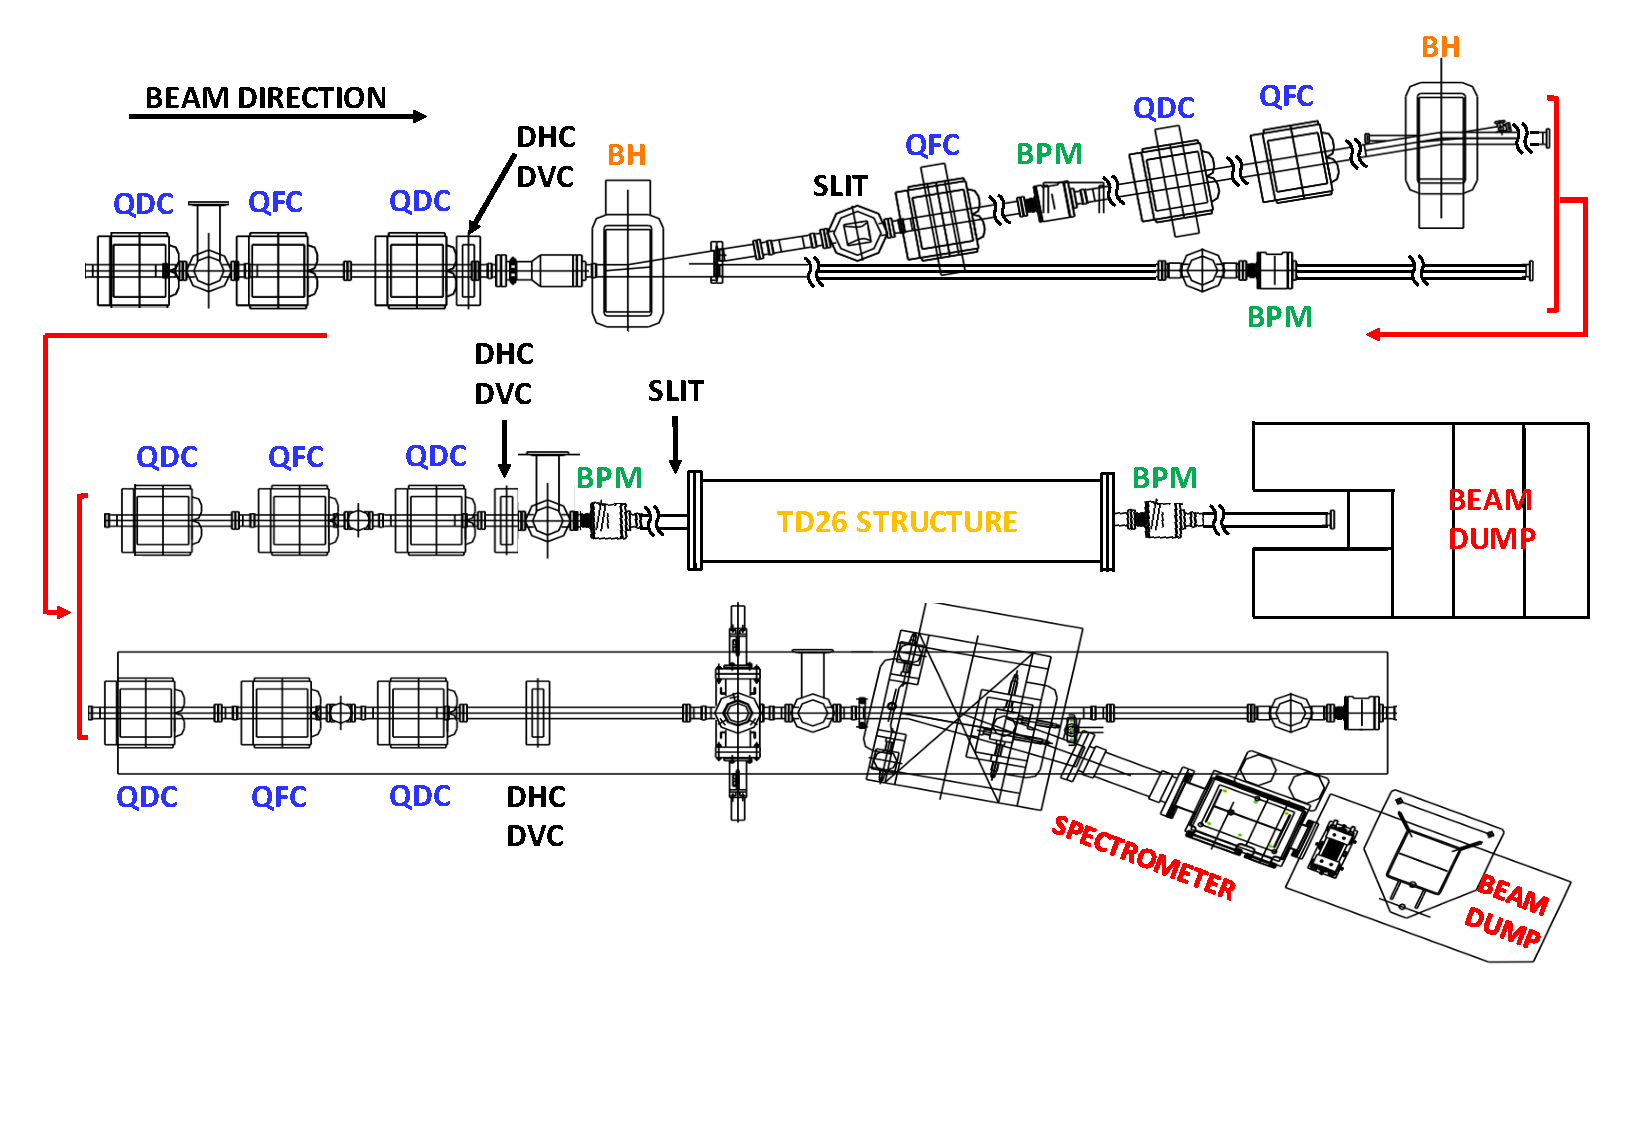
\includegraphics[scale=0.78]{pictures/modified_pets.pdf}
\caption{Simplified layout of optics and beam instrumentation of the dogleg line, adapted from technical drawings and facility layout \cite{EDMS:CTF3}. The beam for this section come from the end of the module 7. Legenda: QFC(QDC): focusing(defocusing) quadrupole; DHC(DVC): horizontal(vertical) dipole corrector; BH: bending magnet in horizontal plane; BPM: beam position monitor}
\label{dolaut}
\end{figure}
\end{landscape}



\subsection[Comparison of setup and CLIC design]{Comparison of setup and CLIC design}



\section[RF power generation]{RF power generation}

The development of the accelerating cavities technology is strongly related to the possibility to produce and test prototypes. This test activity allows to improve the understanding of the scaling laws of the phenomena that limit the performance of the accelerating structures, but also to compare the results of different production and conditioning techniques. 

At CERN the production of 12 GHz RF was carried out just in the CTF3 in the Two-beam modules. These reasons highlighted the necessity of standalone test stands to enlarge the test possibilities. This was realised the first time with the installation of the so called X-Band Test Stand 1 (XBOX1) \cite{Peauger:1287901}. Currently there are three X-band test stands active at CERN simultaneously.

\begin{figure}[h]
\centering 
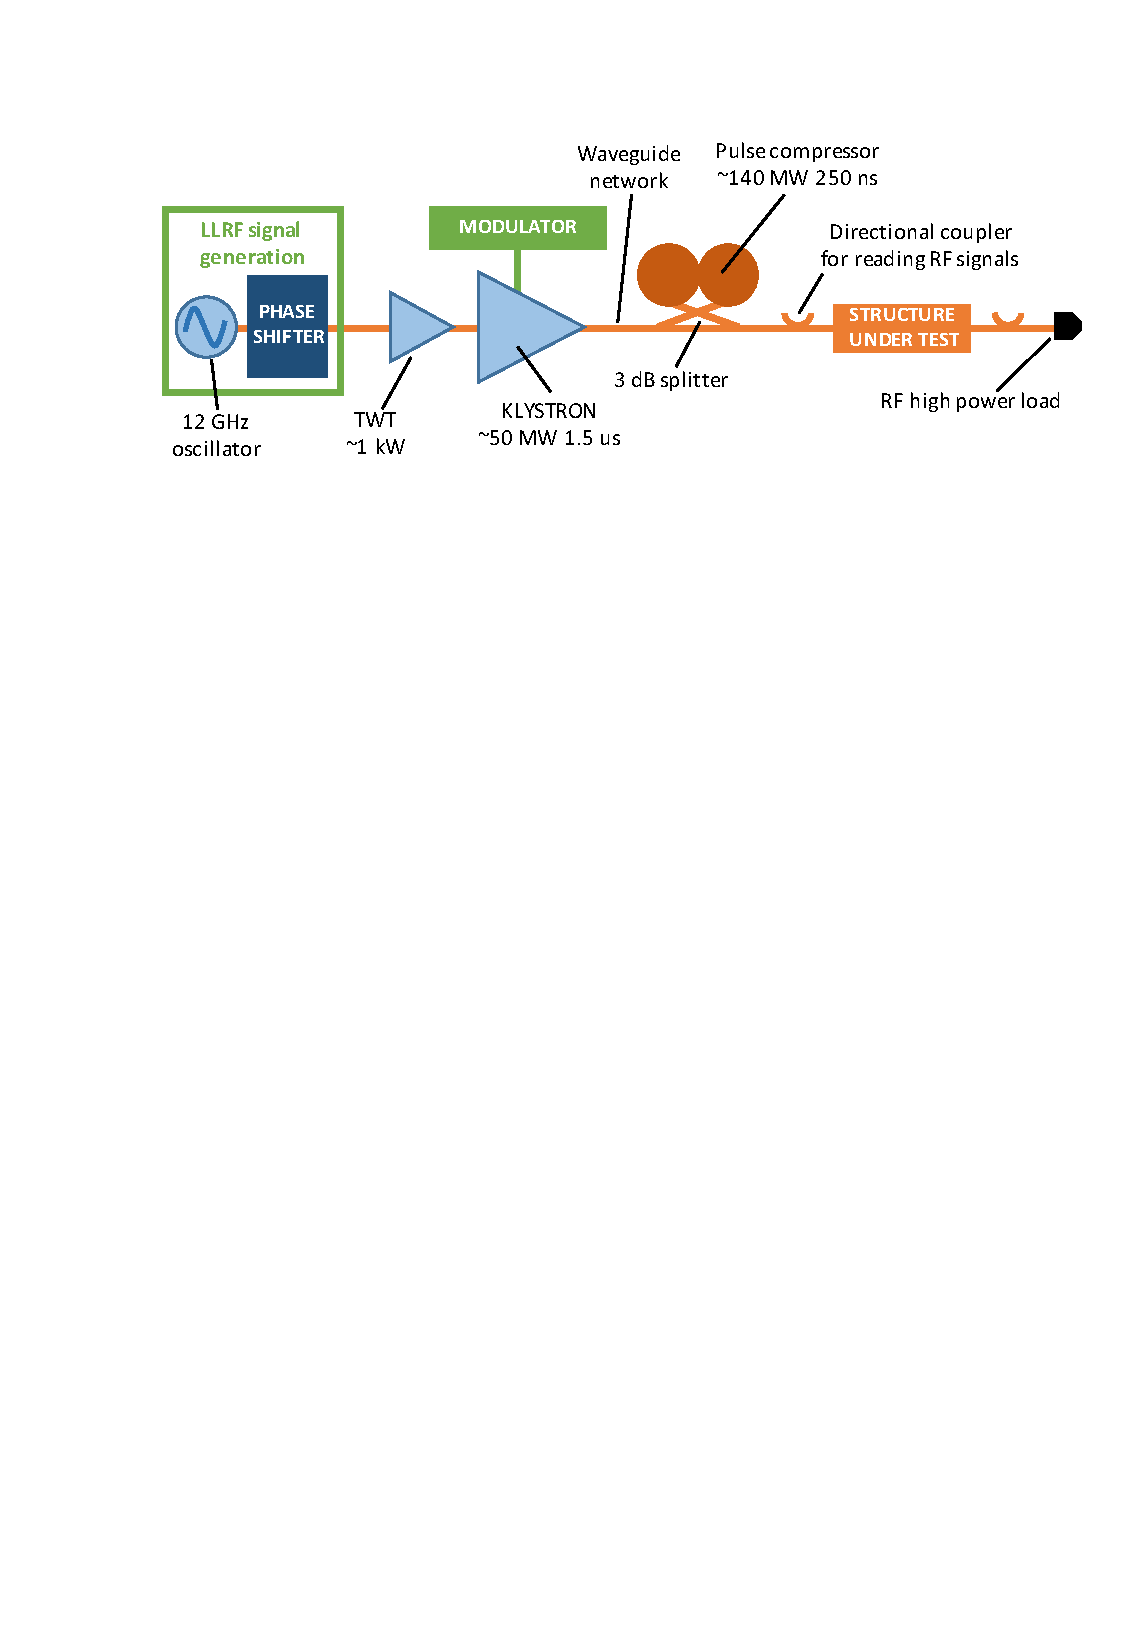
\includegraphics[scale=0.8]{pictures/test_stand_scheme.pdf}
\caption{Standalone X-band test stand layout. Adapted from \cite{Woolley:2015}}
\label{xbox_layout}
\end{figure}

The layout of a RF test stand is shown in figure \ref{xbox_layout}. It is normally formed by signal generation, amplification and delivery systems; diagnostic and control systems, and service systems such as cooling and protection systems. 


\subsection[The X-Box1 at CERN]{The X-Box1 at CERN}

The proposal of an X-band test stand at CERN followed the change of the frequency of CLIC from 30 to the european X-band 12 GHz in 2008. An organic description of XBOX1 is in \cite{Woolley:2015,Kovermann:1459879}. The high-power RF production is realised using:
\begin{itemize}
\item SLAC built XL-5 klystron, able to produce 50 MW of 12 GHz radiation with a pulse length of $1.5\, \mu$s and a repetition rate up to 50 Hz.
\item Scandinova modulator is used to power the klystron.
\item SLED1 type RF pulse compressor is able to compress the klystron output pulse to a shorter one of 140 MW, 250 ns long, which is enough to test accelerating structures considering the waveguide losses.
\end{itemize}

The RF delivery from the pulse compressor to the structure is realised using WR90 waveguides, kept under high-vacuum at a pressure of the order of\\ $5\times10^{-9}$ mbar. In order to reduce the losses, some part of the line to the structure under test is realised with low loss waveguides. This structure requires mode converters because the fundamental modes of the waveguides are different. The overall transmission of the waveguide from the pulse compressor to the structure under test is around 67 \%.

More details regarding the key components of the system are presented in the following sections. The system is controlled solely by the Low-Level Radio Frequency (LLRF), since the gain of the amplification chain is fixed. This feature makes necessary a unique control system of the LLRF together with the Data Acquisition system (DAQ), that will be described in section 4.3.


\subsubsection{TWT, Klystron and modulator}

%missing name of the TWT and check the specs

The very first power amplification stage is carried out by a NAME OF TWT Travelling Wave Tube (TWT), which is a device with the same working principle of the klystron (described below). It is in charge to raise the power of the signal from some watts to up to 3 kW.

XL-5 klystrons comes from the effort made in SLAC to develop high efficiency klystrons for the Next Linear Collider project (NLC). Them are based on the XL-4 klystrons, adapted from the american X-band frequency of 11.4 GHz to the european 12 GHz. This effort lead to the CPI VKX-8311A tubes that are currently in use\cite{klystron:CPI}, which are able to produce a pulse of 50 MW of power, $1.5 \, \mu$s long with an efficiency of the order of 40\%.
 
Klystrons are vacuum tube amplifiers. Are composed of a thermoionic gun, that emits a pulsed beam of electrons. The beam passes through one or several cavities, where a low power RF modulates the beam. After a drift space, where the beam is kept collimated by a solenoid and accelerated by a fixed DC field, the beam passes through a passive cavity that extracts the high power RF. The beam is then dumped. 

The klystron is operated in pulsed mode to enhance efficiency. This means that a power supply able to deliver short pulses of high power is necessary. In the XBOX1 is used a K-3 solid state modulator by Sacandinova, able to supply voltage pulses of 410 kV with currents of the order of 310~A.


\subsubsection{Pulse compressor}

The pulse compressor is the device used to convert the long pulse of the klystron to a shorter one at a higher power. The operation principle is that the power from the klystron is stored in high-Q resonant cavities during the pulse. Before the end of the pulse the cavities are emptied by reverting the phase of the input power. The emptying process is done in a shorter time than the filling one, determining the production of a short high power pulse. 

This technique can lead to the peak power increase up to a factor 5-7. 

The SLED-I type pulse compressor is using two cavities, coupled with a 3 dB hybrid coupler, in order to discharge the produced power to the desired load instead of sending it back to the klystron. The theory is fully described in \cite{Fiebig:209756}, the application in XBOX1 in \cite{SLED:ctf3}.

 


\section[DAQ \& LLRF control systems]{DAQ \& LLRF control systems}

The control system is in charge of generating a phase-modulated signal for the successive amplification stages (TWT and klystron). It also has to acquire the signals from the directional couplers, and the diagnostic signals from the structure and the vacuum systems. According to the diagnostic input, it modulates the signal and can also act on the beam permit of the gun of the linac. 

\subsection[Hardware]{Hardware}

To perform his task, the control system is made of different components, including PLCs (Programmable Logic Controller) interlock systems,  VME (Versa Module Europa) crate based arbitrary signal generators, OASIS PC based digitisers and PXI (PCI eXtension Instrumentation) based control systems.

The core of the system is the National Instrument PXI crate \cite{NI:PXI}, that is the most advanced system in the setup. This carries out: the acquisition and elaboration of all the signals relevant for interlocking the system; trigger the interlocks; save in the internal HDD the recorded signals and retrieve the signals sampled externally in case of an interesting event; interface the rest of the instrumentation.


Since the phase of the LLRF signal has to be modulated to be able to perform the pulse compression, after the generation, the LLRF signal is sent to an analog and a digital phase shifter in series. During the experiments with beam, the digital one is used to phase the beam with the RF feeding the accelerating cavity.

The data acquisition from the -50 dB directional couplers on the waveguides is fulfilled using different kind of sensors:
\begin{enumerate}
\item Diodes with a bandwidth of 500MHz convert the RF signals in a DC voltage level
\item IQ demodulators are used to measure the phase and the amplitude
\item Logarithmic detector are used to acquire the signals with a wide dynamic range of over 46 dB
\end{enumerate}

The PXI crate has 8 channels of 14-bits, 250 MSa/s digitisers. These digitisers are connected to an FPGAs to detect if the signals overcome the critical thresholds. In case the FPGA sends a signal to the trigger unit to interlock the LLRF signal production. A 24 channel Digital Multimeter (DMM) unit is used to read the vacuum signals from the ion pump controllers. The fast digitisers acquire the signals from the logarithmic detectors. 

The signals of the IQ demodulators are sampled by OASIS acquisition PC containing 16 units of 1 GSa/s, 8-bits ADCs. These are read by the PXI crate and archived only during the breakdown events for the offline analysis. 

The signals of the BPMs are acquired and recorded as well by one of the acquisition card of the PXI crate.

%diodes?

%%%Modifications after moving to the dogleg ??? 






\subsection[Online triggers]{Online triggers}

In order to protect the equipments, a number of parameters are constantly monitored and can interlock the setup. Every piece of the equipment has its internal interlocks defined by the constructor. E.g. in the modulator: pressure in the waveguides, door of the higher radiation zone open, internal arc in the klystron, cooling oil system failure, ...; or in the TWT: reflected power out of scale, ... 

The effect of such interlocks is to shut down the affected part, but the rest of the equipment stays on.

A different matter is the interlocking system that is implemented in the PXI crate. When it is triggered, it acts on the LLRF power, cutting the power but leaving the rest of the amplification chain ready. There are four interlocks of this kind, triggered overcoming a user-defined threshold:
\begin{enumerate}
\item {\makebox[7cm]{Peak reflected power:\hfill} $max(P_{REF})$}
\item {\makebox[7cm]{Reflected energy:\hfill} $\int P_{REF}(t) \, dt $}
\item {\makebox[7cm]{Missing transmitted energy:\hfill} $\int P_{INC}(t)\,dt - \int P_{TRA}(t)\,dt$}
\item {\makebox[7cm]{Peak power reflected to the klystron:\hfill} $max(P_{KREF})$}
\end{enumerate}
%is that accurate ? Do the power is always set to zero, even for a BD in the structure?
The last one is again to protect the klystron, and is triggered when the reflected power back from the pulse compressor is too high. This happens especially when the pulse compressor is not properly tuned, as described later in this chapter.
The first three indeed are used to detect a breakdown event inside the structure under test. When one or more of these four interlock is triggered, the event is saved by the PXI crate. If no interlock is triggered in one minute, an event is saved as a backup to monitor the state of the current test.

\section[Other systems]{Other systems}
mention here thermostatic system of the structure and vacuum system ....

Anything else missing ???

\section[Operation of the setup]{Operation of the setup}

- linac switch operation

- pulse compressor issues

- relative phase beam / x-band RF









